% siminos/blog/rpo.tex
% $Author$ $Date$

\documentclass[letter,10pt]{article}

\title{\KS\ blog: \rpo s}
\author{Evangelos Siminos,
    Ruslan Davidchack
    and Predrag Cvitanovi\'{c}, }

\input ../inputs/setupBlog      %% logical chores (nothing to edit)
\input ../inputs/editsDasbuch   %% editing comments, DasBuch style
\input ../inputs/def            %% do not edit; update from dasbuch/book/inputs/def.tex
\input ../inputs/defsBlog       %% all Vaggelis bloggy macros: \renewcommand, etc


\begin{document}

\maketitle

\setcounter{page}{1}
\tableofcontents
\newpage

Throughout:  {\textdollar} on the margin
{\steady}
indicates that the text has been transferred to
article siminos/rpo\_ks/ .

% Enter details, like dates in/out, dated comments into \subsubsection{--project--}
% enter live PDF links to blogs etc where ongoing work is described or forgotten
% continuously reorder items by priority


\input strategy
\input bluesky

\newpage

\section{ES: May 24, 2008 -- Zeghlache Mandel center manifold}

This is just an attempt to understand the primary bifurcation in
Zeghlache and Mandel\rf{ZeMa85} 5-dimensional flow:
\bea
\dot{x}_1 &=&  \sigma (- x_1 -  \delta x_2 + y_1)
               \continue
\dot{x}_2 &=&  \sigma (\delta x_1   - x_2 + y_2)
               \continue
\dot{y}_1 &=& \rho\,  x_1 - y_1 + \delta y_2 - x_1 z
                                                \label{ZMeqs} \\
\dot{y}_2 &=& \rho\,  x_2 - \delta y_1 - y_2 - x_2 z
               \continue
\dot{z}   &=& x_1 y_1 + x_2 y_2  - \gamma\, z
            \,.\nnu
\eea
Here $\sigma>1,\, \rho>0$.

The equation is equivariant under the action of $\Gamma=SO(2)$ defined by
 \beq
 {D}(\theta)
%  =   \left(\barr{ccc}
%     {\bf R}(\theta) &  0              & 0  \\
%     0               & {\bf R}(\theta) & 0  \\
%     0               &  0              & 1
%     \earr\right)
=   \left(\barr{ccccc}
   \cos\theta  &  \sin\theta & 0  &  0 & 0  \\
  -\sin\theta  &  \cos\theta & 0  &  0 & 0 \\
   0  &  0 & \cos\theta  &  \sin\theta & 0  \\
   0  &  0 &-\sin\theta  &  \cos\theta & 0 \\
   0  &  0 & 0  &  0 & 1
   \earr\right)
 \,.
 \label{ZMrotation}
 \eeq

The \stabmat\ is
  \beq
{\Mvar_{ZM}} =
  \left(\barr{ccccc}
    -\sigma    & -\epsilon\sigma & \sigma &  0       &  0 \\
\sigma\epsilon & -\sigma         & 0      & \sigma   &  0 \\
\rho-z         &     0           & -1     & \epsilon & -x_1 \\
0              & \rho-z       & -\epsilon & -1       & -x_2 \\
y_1            & y_2             & x_1    & x_2      & -\gamma
    \earr\right)
\,.
  \ee{ZMstabMat}

The \stabmat\ commutes with ${D}(\theta)$ for points on the fixed point subspace of $\Gamma$, \ie the
$z$-axis.

The origin is a fixed point of the flow and as it is rotationally invariant (lies on the $z$-axis)
its \stabmat\ has no zero eigenvalue associated with the action of $\Gamma$. For $r<1+\delta^2$
the origin is a stable fixed point, while at $r=1+\delta^2$ the stability
matrix has eigenvalues $ \left(0,0,-\gamma ,-(\sigma+1) \pm i \delta  (\sigma-1) \right)$
and  thus a bifurcation occurs which in the literature\rf{GL-Gil07b} is classified as pitchfork to a
stable circle ($\Gamma$-orbit) of equilibria, while the origin looses stability. This is a surprising
fact because generically \rf{golubII} one would expect an equivariant Hopf bifurcation to a $\Gamma$-invariant periodic
orbit, \ie a relative equilibrium (traveling wave). Of course, in view of the degenerate zero eigenvalue
of the \stabmat\ at bifurcation we already begin to question the posibility of a Hopf bifurcation.
Nevertheless one should proceed by first reducing the bifurcation problem to one where all of the \stabmat\ eigenvalues
have zero real part, \ie apply either Lyapunov-Schmidt reduction\rf{golubI} or the Center Manifold Theorem\rf{guckb}.
We follow the latter approach. The procedure is standard but for a five dimensional system I had to use computer algerba
to hope to do it correctly\ES{I only outline the procedure for now, I'll give a better description
and explicit form of transformation matrices, etc, later on if needed.}.

We begin by a linear transformation to new variables $w_i,\, i=1\ldots 5$ such that at bifurcation
the \stabmat\ at the origin is in block-diagonal form. Thus we use the transformation
\beq
	w = T^{-1} x
\eeq
where $w$ and $x$ is shorthand notation for the new and old variables respectively and $T$ is the column matrix of
eigenvectors of \stabmat\ evaluated at the origin, for $\rho=1+\delta^2$. We seek an approximation to the center manifold
as a graph over the center manifold: $w_i = h_i(w_1,w_2,\mu),\, i=3\ldots5$, where $\mu=\rho-1-\delta^2$ is regarded
as the bifurcation parameter but also as an extra variable satisfying $\dot{\mu}=0$. Substituting a Taylor expansion for $h$
up to third order in $w_1,w_2,\mu$ in the transformed equation\ES{actually to a PDE for h which I haven't introduced.} we obtain a local approximation of the center manifold
and we can write the dynamics for $w_1,w_2$ as:
% \begin{eqnarray}
%  \dot{w}_1 & = & \frac{ \sigma}{B^2+F^2}\left[ F\left(\mu +\frac{\left(3 B^2-F^2\right) \mu ^2 \sigma }{\left(B^2+F^2\right)^2}-\frac{w_1^2+w_2^2}{\gamma
%  \left(1+\delta ^2\right)}\right) w_1 + B\left(\mu +\frac{\left(B^2-3 F^2\right) \mu ^2 \sigma }{\left(B^2+F^2\right)^2}-\frac{w_1^2+w_2^2}{\gamma  \left(1+\delta
% ^2\right)}\right) w_2 \right]  \\
%  \dot{w}_2 & = & \frac{ \sigma}{B^2+F^2}\left[ -B\left(\mu +\frac{\left(B^2-3 F^2\right) \mu ^2 \sigma }{\left(B^2+F^2\right)^2}-\frac{w_1^2+w_2^2}{\gamma
%  \left(1+\delta ^2\right)}\right) w_1 + F\left(\mu +\frac{\left(3 B^2- F^2\right) \mu ^2 \sigma }{\left(B^2+F^2\right)^2}-\frac{w_1^2+w_2^2}{\gamma  \left(1+\delta
% ^2\right)}\right) w_2 \right]
% \end{eqnarray}

\begin{eqnarray}
 \left(\begin{array}{c} \dot{w}_1 \\ \dot{w}_2  \end{array}\right) & = & \left[\lambda + g_r(w_1^2+w_2^2) \right]\left(\begin{array}{c} w_1 \\ w_2  \end{array}\right) + \left[\omega + g_\theta(w_1^2+w_2^2) \right] \left(\begin{array}{c} -w_2 \\ w_1 \end{array}\right)
\end{eqnarray}
where
\[\begin{array}{cc}
	\lambda = \frac{ \sigma F}{B^2+F^2} \left(\mu +\frac{\left(3 B^2-F^2\right) \mu ^2 \sigma }{\left(B^2+F^2\right)^2}\right)\,, &
		\omega = -\frac{ \sigma B}{B^2+F^2}\left(\mu +\frac{\left(B^2-3 F^2\right) \mu ^2 \sigma }{\left(B^2+F^2\right)^2}\right) \\
	g_r= -g_\theta= -\frac{ \sigma F}{B^2+F^2} \frac{w_1^2+w_2^2}{\gamma\left(1+\delta ^2\right)}\,,  & B = \delta(\sigma-1)\,,\ F=\sigma+1\,.  \\
\end{array}
\]

In this form it is clear that the reduced system is $SO(2)$-equivariant and that the eigenvalues of the \stabmat\ vanish at the bifurcation. Thus we can't have a Hopf bifurcation. On the other hand, for $\mu>0$ and sufficiently small there is no equilibrium
other than the origin, while there is a $SO(2)$-invariant periodic orbit, \ie a relative equilibrium. This is most readily seen if
we transform the system in polar coordinates:
\bea
	\dot{r} &=&\left(\lambda+ g_r(r^2)\right)r \continue
	\dot{\theta} &=& \omega+ g_\theta(r^2)\,.
\eea
This form justifies the use of $g_r,g_\theta$ above. One can see that we cannot have $\dot{r}=\dot{\theta}=0$ for $\mu>0$ and
thus there are no equilibria to the right of the bifurcation point (other than the origin) . On the other hand there exists a Hopf(?) cycle with
\beq
	r^2= \gamma  \left(1+\delta ^2\right) \mu  \left(1+\frac{\left(3 B^2-F^2\right) \mu  \sigma }{\left(B^2+F^2\right)^2}\right)\,,\ \dot{\theta}=\frac{2 B \sigma^2 \mu^2}{\left(B^2+F^2\right)^2}\,,
\eeq
which is a geometrical circle and thus is $SO(2)$-invariant, \ie it is a relative equilibrium.

This is in direct contradiction with my proof of no existance of relative equilibria in the original system, so something
is wrong. Posibilities are: The application of center manifold theorem was not performed correctly (perharps consider $\delta$
as bifurcation parameter?) One has to go one step further and study the unfolding of the bifurcation (is it codimension-4 bifurcation
or am I counting totally wrong?) I meshed up in proving there aren't relative equilibria in ZM system (did somebody else check at least the polar coordinate representation of the system?) The relative equilibrium in the center manifold is not relative equilibrium in
the original system (sounds crazy but I'll check it.)

\section{ES: April 22, 2008 -- Locating Heteroclinic Connections}

I recently tried to locate heteroclinic connections in Lorenz equations. One
can easily see that the 2-dimensional unstable manifold of $\EQV{1}$ intersects the
$2-$dimensional stable manifold of $E_0$ and thus there should be such connections.
As I couldn't find Predrag's secret method documented somewhere I followed a simple
shooting approach.

Although a heteroclinic orbit is an infinite-time orbit it is sufficient to
pin down a finite time segment of the orbit originating at the linear unstable subspace $E_u^{(1)}$
of $\EQV{1}$ and ending at the linear stable subspace $E_s^{(0)}$ of $\EQV{0}$. Those
requirements can be expressed as the boundary value problem:
\bea
	x(0) & = & \EQV{1}+ \epsilon Re(\mathbf{e}_1^{(1)}) \, \label{eq:shootHetIC} \\
	P_1^{(0)} (x(T)-\EQV{0}) & = &  0 \,. \label{eq:shootHetBC}
%%	P_2^{(0)} (x(T)-\EQV{0}) & = &  d_2 \,. \label{eq:shootHetFixT} %% Not needed for Lorenz
\eea

Eq. \refeq{eq:shootHetIC} imposes the requirement that we start on the unstable subspace of $\EQV{1}$.
Alternatively we could have used as a search space a circle of radius $\epsilon$ on the plane defined
by orthonormalizing $\left(Re(\mathbf{e}_1^{(1)}),Im(\mathbf{e}_1^{(1)})\right)$, parametrized by some
angle $\theta$. Eq. \refeq{eq:shootHetBC} imposes the condition that the final point on the trajectory is
on the stable manifold of $\EQV{0}$. Here
\beq
	P_j^{(0)}= \prod_{i\neq j}^d \frac{\mathbf{A}(\EQV{0})-\lambda_i^{(0)} \mathbf{1}}{\lambda_j^{(0)}-\lambda_i^{(0)}}\,,
\eeq
is projection operator on the $j$'th eigendirection of the linear stability matrix $\mathbf{A}$ at $\EQV{0}$.
%Condition \refeq{eq:shootHetFixT} needs to be imposed due to the time-translational invariance of the
%equations. It corresponds to restricting the final point on a \Poincare section $\PoincS$ transverse to
%the least contracting eigendirection of $\mathbf{A}(\EQV{0})$. For Lorenz this would be a plane normal
%to the $z$-axis at distance $d_2$ from $\EQV{0}$.
\ES{According to Predrag's notation the left hand side
of equation \refeq{eq:shootHetBC} %%and \refeq{eq:shootHetFixT}
is a scalar.}

To solve the boundary value problem I have used Newton's method to refine a guess for $\epsilon_n$. %and $T_n$
%based on the linearization:
%\beq
%	f^{T_{n+1}}(x_{n+1}) \simeq f^{T_n}(x_n) + \mathbf{J}^{T_n}(x_n) Re(\mathbf{e}_1^{(1)})\delta\epsilon\,, %+ v(f^{T_n}(x_n)) \delta T
%\eeq
%and imposing condition \refeq{eq:shootHetBC} % and \refeq{eq:shootHetFixT}
%on $f^{T_{n+1}}(x_{n+1})$.
Predrag suggests using the linear approximation of the flow to analytically continue the heteroclinic
orbits after period $T$ and impose the condition that this analytic solution ends up on the equilibrium.
I cannot see why this is necessary here. The condition \refeq{eq:shootHetBC} guarantees that the solution
is on the linear approximation of the stable manifold of $\EQV{0}$ and thus will end up on $\EQV{0}$.
Essentially this is the analytic part of the problem and no more needs to be done. The accuracy of the
method is limited by the approximation of the local stable manifold of $\EQV{0}$ and the local unstable
manifold of $\EQV{1}$ by the corresponding linear unstable subspaces, \ie by planes in the case of Lorenz
equations. One can estimate the distance of minimum approach to $\EQV{0}$ by using the expressions for
the linearized flow. Disregarding the strongly contracting eigendirection $e_3^{(0)}$ I find:
\beq
	r_{min}^2= d_2^2\left(1-\frac{\lambda_2}{\lambda_1}\right)\left(\-\frac{d_1^2 \lambda_1}{d_2^2\lambda_2}\right)^{-\frac{\lambda_2}{\lambda_1-\lambda_2}}
\eeq
where $d_1=P_1^{(0)} (x(T)-\EQV{0})$ and $d_2=P_2^{(0)} (x(T)-\EQV{0})$ \ES{Predrag might want to compare
this against his secret notes.}. I use this to compare with the actual minimum distance from $E_0$ and
evaluate the validity of the linear approximation of the stable manifold.

In \refref{FriedmanDoedelConnections91} the authors present a
method for computation and continuation of heteroclinic
connections similar in spirit but in a more general setting.
They suggest that a condition breaking the time-translational
invariance should be used along with \refeq{eq:shootHetBC}.
Here, \refeq{eq:shootHetIC} is formulated in a way that
excludes variation in the initial conditions in the direction
of the flow and we need not impose an extra condition.

It works well for Lorenz equations but fails to converge for ZM.

\section{May 17, 2007 -- $s_1$, $s_2$, $\tau_x$, $\tau_z$ generate 16 irreps?}

{\bf PC}: My main problem is - we are currently using only 4 irreducible reps
of $C_2 \times C_2$ = $D_2$ dihedral group generated by $\tau_x, \tau_z$,
but why not 16 irreps of
the $D_2 \times D_2$ generated by $s_1, s_2, \tau_x, \tau_z$?
They all commute, each one splits the space of reps into 2.
Why stop at $U_S$ subspace?
There should be 16 discrete copies of any
general solution, not just 4.
However, there would still be 4 copies of UB, as UB is within the
fully symmetric irrep $A_1$ od $s_1, s_2$ $D_4$.

\section{Jun 13, 2007 Reading for Ruslan?}

Armbruster {\em et. al} showed that four complex Fourier
modes suffice to exhibit most
of the qualitative features of the dynamics,
for a wide range of system sizes\rf{AGHks89}.

\subsection{PC Nov 28, 2007: Japanese heresy}

We do not want to refer to wrong papers, but here it is, for
the internal record, so we do not forget not to cite it
(from Physical Review Letters, 16 Sep 2004 request to referee,
which I ignored):

Mitsuhiro Kawasaki and Shin-ichi Sasa,
    ``Statistics of unstable periodic orbits of a chaotic dynamical system
    with a large number of degrees of freedom."


\section{Symmetry-Reduced Representation (SRR) for KSE}

\subsection{RLD Jan 17, 2008 -- How to quotient the SO(2) symmetry}

In order to quotient the SO(2) symmetry we need to be able to define,
for any state of the KS system $u(x)$
($a = (a_1, a_2, \ldots)^\mathsf{T}$ in Fourier space),
a 'shift' parameter, $s(a) \in S^1 $, such that
\[ \tau_{-s(a)} a \in M/\mathrm{SO}(2). \]
This parameter must satisfy the following {\em monotonicity condition} with
respect to the translation of the state $a$:
\[ s(\tau_{\ell/L}a) = s(a) + \phi(\ell/L) \]
where $\phi(x): S^1 \mapsto S^1$ should be a continuous strictly monotonic function.
This condition is necessary to avoid any ambiguity in the definition of
the shift parameter.

This condition is clearly satisfied when $s(a)$ is proportional to
the first Fourier mode (provided that $|a_1| > 0$)
\begin{equation}
  s(a) =  \theta_1/(2\pi) = \arg(\hat{e}_1^\dagger\,a)/(2\pi)
\label{eq:shift1} \end{equation}
where $\hat{e}_1 = (1+0i, 0, 0, \ldots)^\mathsf{T}$ is the basis vector corresponding
to the first Fourier mode and $\dagger$ denotes Hermitian transpose.
In this case
\[ \arg (e_1^\dagger\,\tau_{\ell/L}a)/(2\pi) = \theta_1/(2\pi) + \ell/L\,, \]
and so $\phi(x) = x$.

It is also possible to get a well-defined shift parameter by
using the difference between phases of Fourier modes $k$ and $k+1$ (provided
that $|a_k|, |a_{k+1}| > 0$):
\begin{equation}
  s(a) = \arg(\hat{e}_{k+1}^\dagger\,a)/(2\pi) -
  \arg(\hat{e}_{k}^\dagger\,a)/(2\pi)\,.
  \label{eq:shiftk} \end{equation}
Maybe for $L = 22$, where dominant Fourier modes are 2 and 3, it is better to use
this shift parameter with $k = 2$?  This needs to be explored.

Of course, as suggested by Predrag, we can define in a similar
fashion the shift parameter with respect to any other
state (e.g. an equilibrium state $a_q$):
\[ s(a) = \arg(a_q^\dagger\, a)/(2\pi)\,, \]
but this shift cannot be guaranteed to satisfy the
monotonicity condition for all $a$.

Since equilibria E1, E2, and E3 for $L = 22$ have dominant
1st, 2nd, and 3rd Fourier modes, respectively, fixing the modes by
Eqs.~(\ref{eq:shift1}) or (\ref{eq:shiftk}) also fixes the equilibria.


\subsection{PC Jan 17, 2008 -- Monotonicity?}

Not sure about need for monotonicity - one needs it for the 1-dimensional
Lie group of time evolution, parameterized by a continuous parameter $t$
which can be conjugated to any other parameter $u = u(t,\ssp)$ as long
as it is monotone, but rotations can go whichever way they want, modulo
$2\pi$ (or $L$). Once we look at a problem with $SO(3)$ symmetry, what's the
need for monotonicity in Euler angles, \etc.?

\subsection{RLD Jan 17, 2008 -- I think we need it...}
Let's say $s(a)$ is defined in such a way that it is not monotonic with respect to
shifts of state $a$.  Then there could exist $\ell_1$ and $\ell_2 \neq \ell_1$ such that
\[ s(\tau_{\ell_1/L}\,a) = s(\tau_{\ell_2/L}\,a) = s\,. \]
Then $\tau_{\ell_1/L - s}\,a$ and $\tau_{\ell_2/L - s}\,a$ would be two distinct points
in $M$/SO(2) representing the same state $a$.  This doesn't seem right.

\subsection{2009-08-26 RLD: back to epicycles}
%{\em \underline{Preamble:} My gut tells me that the method of moving frames, as described in the Section 4.2 of the thesis will \underline{not} work for KS.  But since my brain is dafter than my gut, I cannot explain why I feel that way.  So, in order to make progress in this direction, I'm going to work with a dynamical system similar to KS, but much simpler.  If I can figure out how to apply the moving frames to this system, then I can do it for KS as well.  If not, then I hope it will help me understand why my gut is right. \vspace{2ex}}

\noindent{\bf Ruslan:} Forget \KS, let's consider a simpler dynamical system.
Let's say that, just like KS, we have a dynamical system on the space of real function $u(x,t)$ periodic in $x \in [-\pi, \pi)$, i.e. $u(x+2\pi,t) = u(x,t)$.  In the Fourier space $a = \mathcal{F}[u]$, $a = (a_1, a_2, \ldots)$, $a_k \in \mathbb{C}$ and $a_{-k} = a_k^\ast$.
I will also use polar coordinates, so $a_k = r_k \mathrm{e}^{i \phi_k}$.
The action of $U(1)$ on $u(x,t)$ is $g(\theta) u(x,t) = u(x+\theta,t)$. In the Fourier space
\[ g(\theta) a_k = \mathrm{e}^{ik\theta}a_k\,, \]
%In polar coordinates $\tau_{\ell/L} (r_k, \theta_k) = (r_k, \theta_k + q_k \ell)$.
To define the $U(1)$ group rotation tangent $t(a)$, we consider an infinitesimal rotation
\[ \mathrm{e}^{ik\theta}a_k = (1 + ik\theta)a_k  = a_k + \theta t_k\,, \]
so $t_k = ika_k$.
    \PC{I do not understand this, so I removed it:
    ``We can also define $\mathbf{T} = \mathrm{diag}(ik)$,
    so that $t = \mathbf{T}a$.''}

The equation defining the slice through some point $a^*$ is
    \PC{Will have to redefine $a^*$, $t^*$, it conflicts with complex conjugation
        for $U(1)$.}
\[ (\bar{a} - a^*) \cdot t^* = 0 \]
By the dot product we mean
\[ a \cdot b = \sum_{k=-\infty}^\infty a_k b_k^*\,, \]
which in the space of periodic functions corresponds to
\[ f \cdot g = \int_{-\pi}^\pi f(x) g(x) dx\,, \]
where $f(x) = \mathcal{F}^{-1}[a]$ and $g(x) = \mathcal{F}^{-1}[b]$, so this makes sense.  But note that this is not the only way of defining the dot product...

\subsubsection{Epicycles: 2-Fourier modes linear dynamical system}

Let's define the dynamical system $\dot{a}_k = v_k(a)$ as follows:
$v_k = i \omega_k a_k$, $\omega_{-k} = -\omega_k$,
where $\omega_k \in \mathbb{R}$ are constants.
    \RLD{$\omega_{-k} = -\omega_k$.
    I used this in my derivation to get the sign right.
    {\bf Predrag:} Agreed - I used that too in rederiving your model.}
This is a linear dynamical system, so we can solve it analytically:
\[ a_k(t) = a_k(0) \mathrm{e}^{i \omega_k t} \]
Even simpler, I'm going to use only the first two modes, so $a_k(0) = 0$ for all $|k| \neq 1$ or 2.

We can choose constants $\omega_1$ and $\omega_2$ such that this system can have
a traveling wave or a RPOs in the original space of periodic functions $u(x,t)$.\\
{\bf Example 1:} If $\omega_1 = c$ and $\omega_2 = 2c$, then
\[ a_k(t) = a_k(0) \mathrm{e}^{ikct} = g(ct) a_k(0)\,, \]
which is a wave traveling with speed $c$.\\
{\bf Example 2:} For the system to have an RPO, we can choose, for example,
$\omega_1 = \pi/2$ and $\omega_2 = 3\pi$.  This RPO has period $T = 1$ and shift $\pi/2$, since
\[ a_1(1) = a_1(0) \mathrm{e}^{i\pi/2} = g(\pi/2) a_1(0) \quad \mathrm{and} \quad
   a_2(1) = a_2(0) \mathrm{e}^{i3\pi} = a_2(0) \mathrm{e}^{i\pi} = g(\pi/2) a_2(0) \]

Let's now see what happens if we apply the method of 'slices' to these two examples.  The reconstruction equation is
\[ \dot{\theta} = \frac{v(\bar{a}) \cdot t(a^*)}{t(\bar{a}) \cdot t(a^*)} \]
Let's say the initial condition $a_1(0) = r_1 > 0$, $a_2(0) = r_2 > 0$ (i.e. $\phi_1 = \phi_2 = 0$) is also the point $a^*$ defining the slice.  Then
$t_k(a^*) = ikr_k$ when $|k| = 1,2$ and zero otherwise.  So,
\beq
\dot{\theta} = \frac{\sum_k (i\omega_k \bar{a}_k) (ikr_k)^*}{\sum_k (i k \bar{a}_k)(ikr_k)^*}
                = \frac{\sum_k k \omega_k \bar{a}_k r_k}{\sum_k k^2 \bar{a}_k r_k}
\ee{RLDrec}
The equation for the flow on the slice (aka reduced flow) is
    \PC{have this also for $a^*$ complex, if we need it - no reason to chose
        it real, though it seem not to be the cause of the singularity in $\dot{\theta}$
        }
\beq
\dot{\bar{a}}_k = v_k(\bar{a}) - \frac{v(\bar{a}) \cdot t(a^*)}{t(\bar{a}) \cdot t(a^*)} t(\bar{a})
                   = i\omega_k \bar{a}_k - \frac{\sum_k k \omega_k \bar{a}_k r_k}{\sum_k k^2 \bar{a}_k r_k} ik\bar{a}_k\,.
\ee{RLDred}
\noindent {\bf Example 1:} Here $\omega_k = kc$, so we immediately get
\[ \dot{\theta} = c \quad \mathrm{and} \quad \dot{\bar{a}}_k = 0\,, \]
as expected for the traveling wave.\\
{\bf Example 2:} In general, for the flow with two non-zero modes (remembering that $a_{-k} = a_k^*$ and $\omega_{-k} = -\omega_k$):
\[ \dot{\theta} = \frac{\omega_1 r_1 (\bar{a}_1 + \bar{a}_1^*) + 2\omega_2 r_2 (\bar{a}_2 + \bar{a}_2^*)}{r_1(\bar{a}_1 + \bar{a}_1^*) + 4r_2 (\bar{a}_2 + \bar{a}_2^*)} \]
and
\[ \dot{\bar{a}}_k = i\omega_k \bar{a}_k - \frac{\omega_1 r_1 (\bar{a}_1 + \bar{a}_1^*) + 2\omega_2 r_2 (\bar{a}_2 + \bar{a}_2^*)}{r_1(\bar{a}_1 + \bar{a}_1^*) + 4r_2 (\bar{a}_2 + \bar{a}_2^*)}ik\bar{a}_k \]
When $\omega_1 = \pi/2$ and $\omega_2 = 3\pi$, the second equation should generate a periodic orbit with period $T = 1$, while the solution of the first equation, starting with $\theta(0) = 0$, should give us $\theta(1) = \pi/2$.  Unfortunately, we cannot solve these equations analytically, so I'll do it numerically for different values of $r_{1,2}$.  I'll set $r_1 = 1$ and increase $r_2$ from zero.  Note that when $r_2 = 0$, we just have a traveling wave with speed $\omega_1$.  Also, when $r_2$ is sufficiently smaller than $r_1$, we will have a traveling wave slightly modulated by the 2nd mode.  This case is shown in the figure below:

\vspace{2ex}\noindent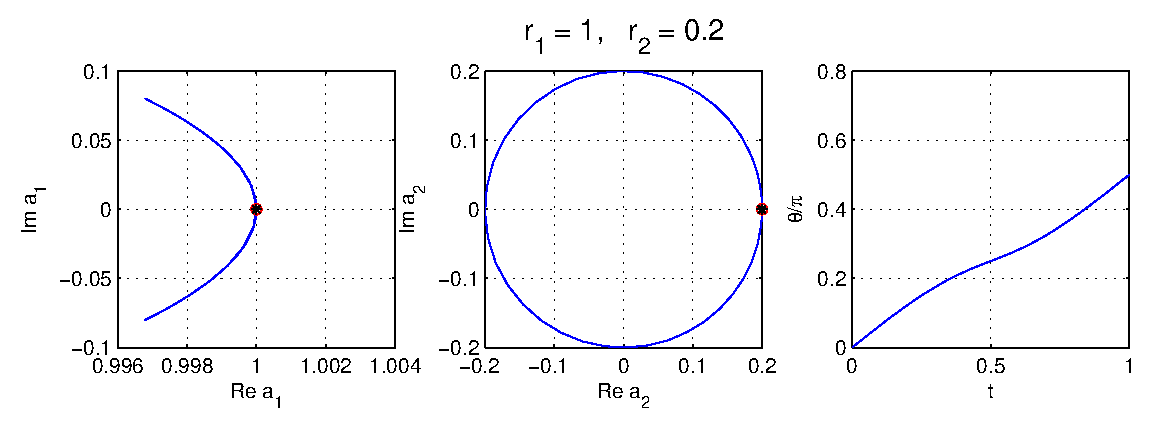
\includegraphics[width=\textwidth]{sliceflow1.eps}

So, everything works well: the reduced orbit is periodic (the beginning of the orbit is denoted by the red circle, while the end is denoted by the black asterisk), and the phase shift at $t = 1$ is equal to $\pi/2$.  We can see similar picture when we increase $r_2$:

\vspace{2ex}\noindent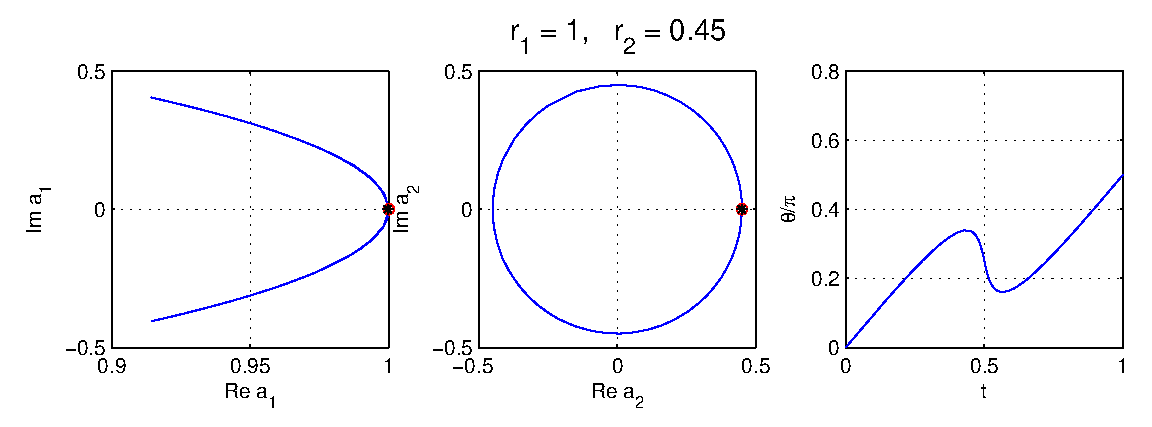
\includegraphics[width=\textwidth]{sliceflow2.eps}

Now, when $r_2$ approaches 0.5, it is clear that the orbit approaches a singularity:

\vspace{2ex}\noindent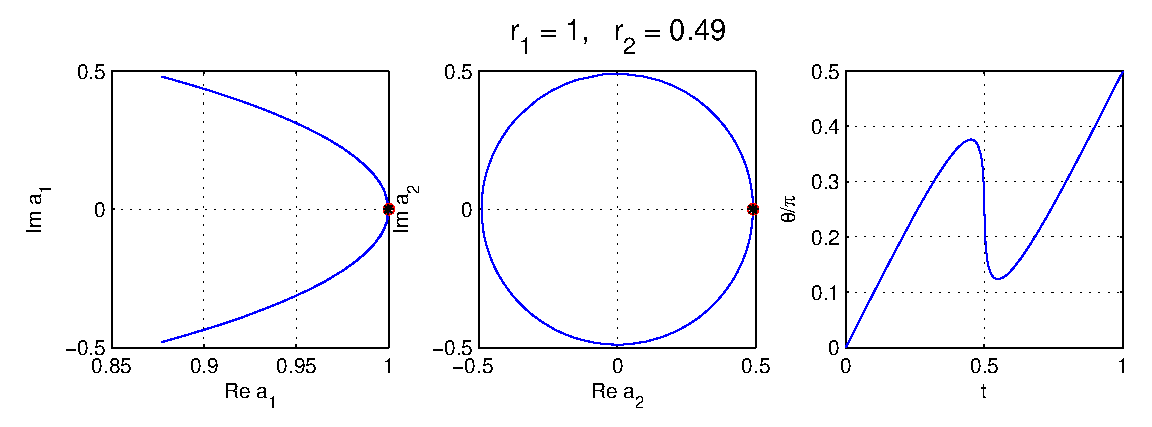
\includegraphics[width=\textwidth]{sliceflow3.eps}

At $r_2 = 0.5$ we get rubbish:

\vspace{2ex}\noindent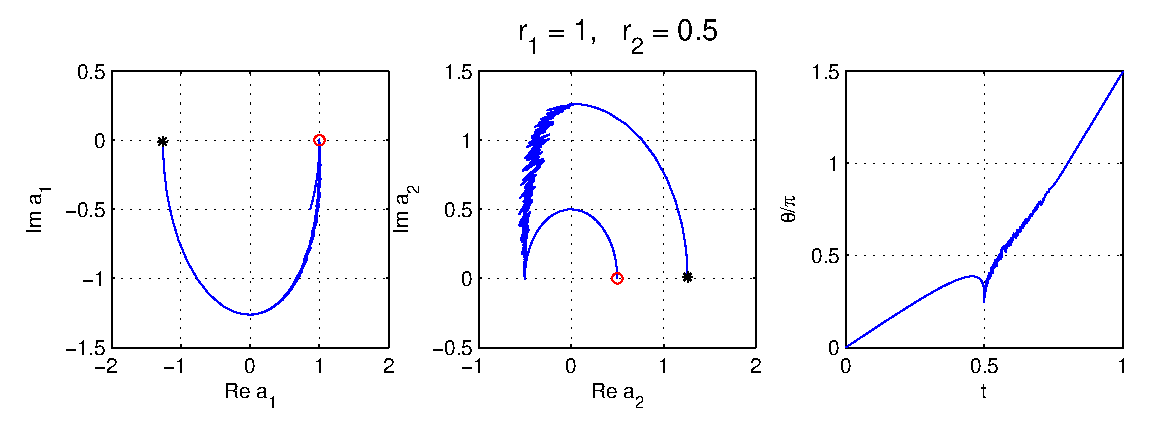
\includegraphics[width=\textwidth]{sliceflow4.eps}

which persists for awhile

\vspace{2ex}\noindent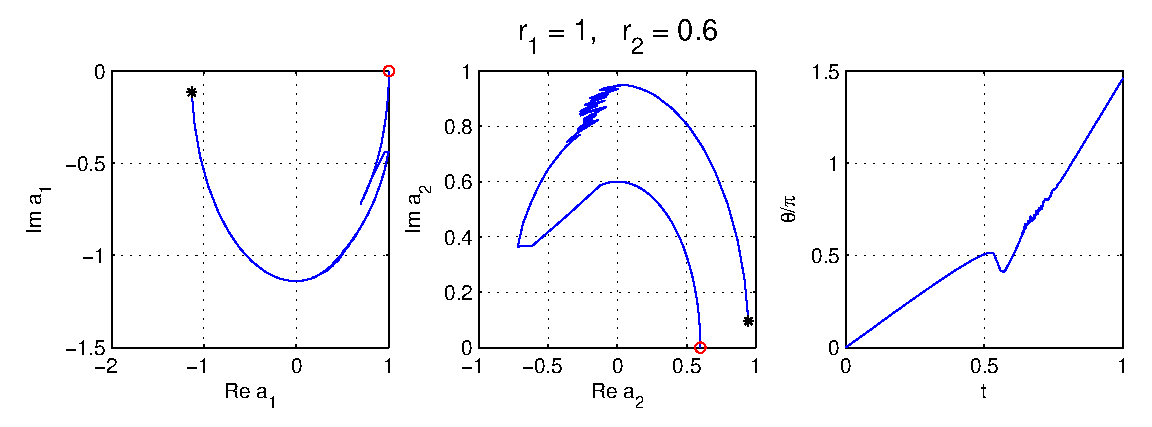
\includegraphics[width=\textwidth]{sliceflow5.eps}

until we get back the nice smooth solution:

\vspace{2ex}\noindent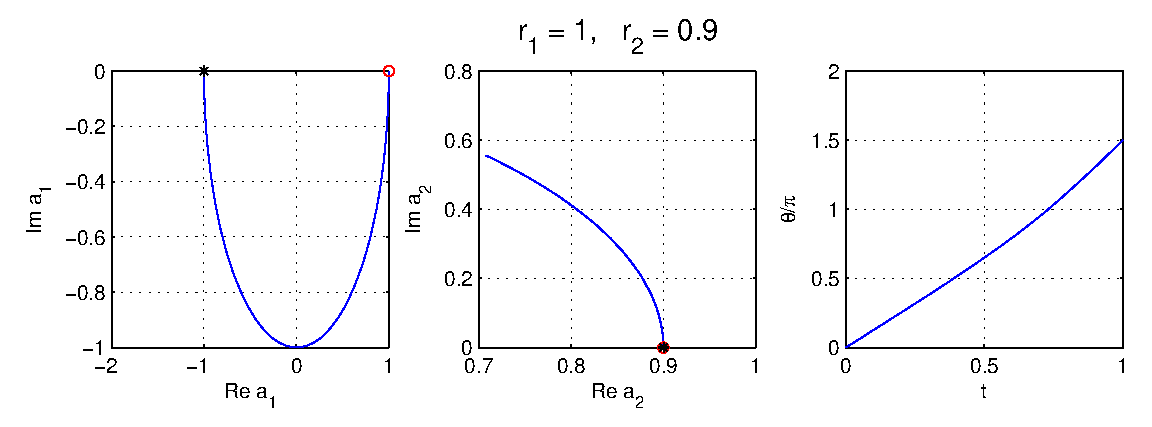
\includegraphics[width=\textwidth]{sliceflow6.eps}

which, however, is no longer periodic, while the shift is now $3\pi/2$.  This picture persists for all $r_2 > r_1$.

\vspace{2ex}\noindent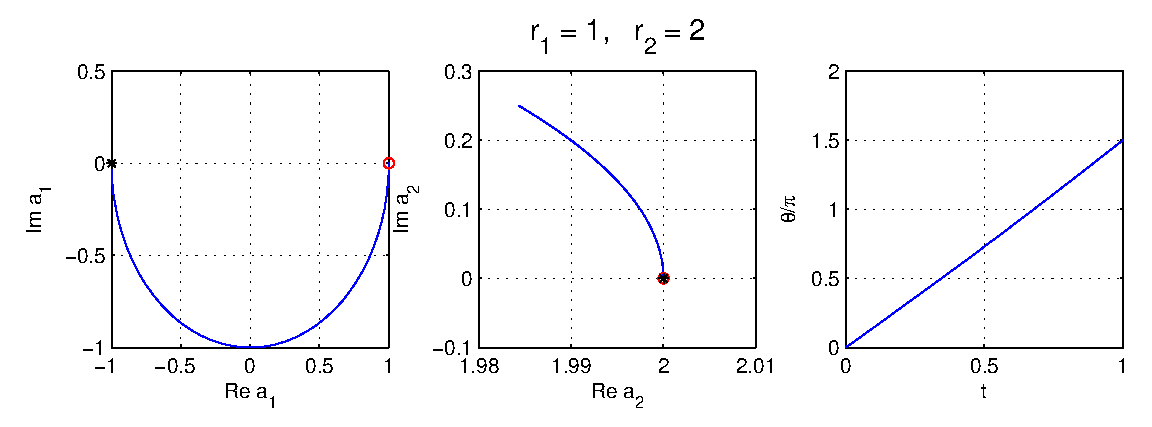
\includegraphics[width=\textwidth]{sliceflow7.eps}

So, it looks like the problem with the method of slices is not only due to running into the singularities, but also due to the possibility of generating smooth orbits which go around those singularities and generate wrong shifts without any indication that something has gone wrong.  These orbits are no longer periodic in the reduced space.  The only time this method works reliably is when the flow is dominated by the first Fourier mode.  If this is not the case, as in the KSE regime with multiple active modes, then we cannot expect that it will work.~~{\em Q.E.D.}

\vspace{2ex}
An old idea presented as a new one:  Why don't we define the dot product in the above equations as follows:
\beq
 a \cdot b = a_1 b_1^* + a_1^* b_1
 \,.
\ee{RLDfix}
Then, if I'm not mistaken, the whole thing reduces to my original idea for factoring out the $U(1)$ symmetry from the KS flow.  In this case we won't need to worry about running into, or moving around, the singularities while generating spurious phases.  The only singularity will be at $r_1 = 0$, which is trivial to deal with.

With the dot product defined as in \refeq{RLDfix}, Eqs.~(\ref{RLDrec}) and (\ref{RLDred}) become
\[
  \dot{\theta} = \omega_1
  \quad \mathrm{and} \quad
  \dot{\bar{a}}_k = i(\omega_k - k\omega_1) \bar{a}_k\,.
\]
So they obviously do the job.


\subsection{2009-08-25 Eurosceptics do not like to slice}
\noindent{\bf Ruslan:} (Predrag's translation) one gets a phase shift by $\pi$ if one crosses the singularity.\\
{\bf Ruslan:} The shifts by $\pi$ is the least of my worries.  It is the fact that when $r_2 > r_1$ we get a nice smooth solution of the reconstruction and reduced equations, yet we get obviously wrong results.  I don't want to think why this is happening.  I'd rather just stop using the approach where such a thing can happen.\\
{\bf Predrag:} Your model illustrates why we need
monotonicity in phase (we are integrating 1d equation,
velocity cannot change sign?). But I think we will fix it -
it is like WKB for harmonic oscillator, one gets geometric
$\pi$ phase for each turn, and a neat way to do it is Maslov
trick - change slice at $\pi/4$, then change back at
$3\pi/4$, etc. Looks like something we can figure out. Sure
cute - getting semiclassical Keller-Maslow phase without
doing neither wave nor quantum mechanics. At least, not
consciously.

More interesting will be the phase for the method of
connections. If we are lucky, it is the same for relative
periodic orbits.\\
{\bf Ruslan:} We had the discussion about monotonicity some
time ago (see above).  I don't have anything more to add at
the moment.\\ I don't know much about WKB, or Keller-Maslow
phase, but I would like to get away from generating all kinds
of fixes, like using random $a^*$ or switching between
slices.

\noindent{\bf Predrag:} 1st mode will not work. Actually,
what Ruslan has run into so far is the same problem you
(Vaggelis) and Rebecca run into independently; he is
measuring angle in polar coordinates, where we also run into
$d\theta/dt$ divergence, and shifts by $\pi$.\\
{\bf Ruslan:} I disagree that 1st mode won't work, I think it
will. And I don't think using polar coordinates is the
problem.  Forget about dynamics.  Just look at functions
defined on a circle and ask yourself how to identify
functions that differ only by a shift.  My answer: The phase
of the 1st Fourier mode will give you the shift.  So just use
it to rotate the functions on top of each other.

\noindent {\bf Vaggelis:} Apart from quantum mechanics there
are classical systems that exhibit such behavior, see for
example
\HREF{http://prl.aps.org/accepted/L/cf079Ya5Q7f19828e08c7183313c1d9b2e9126ce4}
{this PRL paper}. I've only seen it in Hamiltonian systems,
where this behavior is called monodromy since one studies the
system as it goes once around a singularity (is the etymology
clear to non-Greeks too?). It apparently arises when a
function fails to be single-valued, which again should point
out why we need monotonicity in phase.\\
\textit{Question for Ruslan:} Is it really trivial to deal with the singularity at $r_1=0$?\\
{\bf Ruslan:} Yes, but you should never ever try to numerically integrate the reconstruction or the reduced flow equations if you expect to get the correct reduced representation of the orbits of the original flow.  Instead, integrate the original flow and then pull the obtained orbit onto the slice while keeping track of the shift you generate while doing it.  If the original orbit goes exactly through $r_1 = 0$ (within the round-off error), then add (or subtract) $\pi$.  That's all.\\
{\bf Vaggelis:}  \ESedit{I agree that integrating the equation on the slice is not the safest think to do. I would like to understand where the spurius shifts that you have discovered come from, though. It looks like the reduced space has a branch cut and as one integrates the equations around the singularity he finds oneself on a different leaf.

There is something I don't understand in the procedure you describe here. Does the need to add or subtract $\pi$ come from the fact that most
implementations of $arg$ or $arctan$ functions do not distinguish quadrants? I do not understand how else it is connected to crossing through $r_1 = 0$ or why
it does take care of the singularity. You can approach the singularity through any direction on the $a_1$ plane, so the way to overcome the singularity on a point
with $r_1=0$ seems to be to use the angle at which you approach to it (that you get from the previous point) to correctly rotate it onto the slice. The difficulty
is that then you are not able to tell where $\EQV{2}$ and $\EQV{3}$ lie on this space as they both have $r_1=0$: their group orbits do not intersect your slice, so
you do need another ``coordinate chart'' to cover the space.
}\\ %end ESedit
{\bf Vaggelis:} You still need to cover the reduced space with more than one coordinate systems which is essentially the same as choosing a new slice.\\
{\bf Ruslan:} No. You don't need more than one coordinate system.  Just use the Fourier modes as reduced coordinates, with the phase of the 1st mode fixed.  The phase of the 1st mode will be the reconstruction shift.\\
{\bf Vaggelis:} Even if this doesn't bother us, I am afraid that we will get projections that are not more informative than Figure 42 in todays version of my thesis, where the singularity was dealt with but $E_2$ and $E_3$ collapse to the same point.\\
{\bf Ruslan:} I cannot guarantee that the pictures we get will be nice and simple.  Of course, since the reduced space is a semi-space (because $r_1 \geq 0$), the reduced orbits may not always look pretty and smooth: They will have sharp turns when they come close to, or hit, the $r_1 = 0$ subspace.  But at least when I look at orbits projected onto Fourier modes, I know how to interpret them.  When I'm looking at the projections onto some exotic curvilinear coordinates, the pictures make no sense to me.\\
{\bf Vaggelis:} \ESedit{On the utility of Fourier modes as a representation I disagree in two levels. I anyway find that Fourier modes projection tell us very little about dynamics. Wasn't this the reason to use different coordinate systems in the KS paper? So as long we can construct dynamically meaningfull projections in the new variables I do not worry how we got them.

Furthermore, what you describe above is equivalent to using the invariants of Table 3 in Chapter 8 in my thesis. The new coordinates are exactly the Fourier modes rotated back to the slice defined by $Im(c_1)=0$, this is how they were obtained. The difference is that in Table 3 the singularity is explicit. The important point though is that what you like to see as a linear transformation is in fact a nonlinear transformation through the dependance of the angle on the point in space in which it is evaluated. Whereas in a linear transformation all points in space are rotated by the same angle. Therefore without knowing it you use exotic curvilinear coordinates. The connection to the original Fourier modes is that the magnitude in each Fourier plane stays invariant. Of course things get even more exotic in my thesis, but the motivation behind that was to get projections that provide more information about the dynamics.

As a general comment, it appears that when we try to see the reduced space as embedded in the original space, no matter how we go from $N$ to $N-1$ dimensions we impose a conservation law that did not exist in the original system (as it was allowed to have motion in the direction of group action) that restricts the motion to an $N-1$ dimensional space which cannot in general be given a nice structure.
}%end ESedit


\subsection{2009-08-26 Eurosceptics carry the day}

\noindent{\bf Predrag:} OK, now that Ruslan has gone on
strike I spent a day screwing around with Mathematica,
checked epicyclist formulas and reproduced Ruslan's graphs.
As I am using \texttt{NDsolve[\dots]} as a black box, I do
not get the same screwy details close to $(r_1,r_2)=(1,0.5)$,
but the result is the same - for $r_2$ sufficiently larger
than 1/2 one gets extra $\pi$ shift, with no integration hint
that one is going around a singularity. That is unacceptable.
As Ruslan expects,
random choices of complex (not real) slicing section fixing
point $a^*$ move the singularity around but are essentially no
help.

I will still try to use Maslov trick and switch the slice
whenever $\dot{\theta}$ starts misbehaving, but for that I need to learn how
to use \texttt{Method -> \{"EventLocator"} within \texttt{NDsolve[\dots]},
but that sure looks like a bitter pill. I do not mind having several slices
as long as the returns to (dynamical) Poincar\'e sections trace out
smooth unstable manifolds suitable to partitioning the \reducedsp.

Marsdenites did not note this problem as they only applied the method to
\reqva, and there it is OK.

I agree that if one is to fix the \slice\ by one Fourier mode, \refeq{RLDfix} is
the most natural choice, and would be easiest to explain in a publication.
Unfortunately, we ran into singularities when we tried it for
\CLe\ in Siminos thesis\rf{SiminosThesis} and Rebecca's summer project. But Ruslan,
do give it a try.

\noindent{\bf Ruslan:}
Actually, not really on strike, just reluctant to participate
in your, what I believe to be, futile efforts to apply all
kinds of fixes and patches to the approach which, I believe,
is fundamentally incurable when it comes to systems like KS
in a fully developed chaotic regime. [\dots]

\noindent{\bf Predrag:} Fair enough - way too many fixes and
patches. We need to quotient the symmetry in order to figure
out the symbolic dynamics for KS and for plane Couette and
pipe flows. If something like \refeq{RLDfix} works it would
be nicer. The reason why we think it will not is that when we
use the polar coordinates-inspired \slice\ fixing point
$\ssp^{*}=(0+i,0, \cdots)$, $\Re\ssp_1=0,\;\Im\ssp_2>0$
(which I believe for $U(1)$ version corresponds to fixing the
phase of the first Fourier mode) the \reducedsp\ equations
are given by
\beq
\dot{\ssp} = v - \frac{\Im v_1}{\Re\ssp_1} t(\ssp)
\,.
\ee{EqMotionMovFrame}
Trajectories shown in %\reffig{fig:PCunrot1}
Siminos thesis\rf{SiminosThesis} and Rebecca's summer project
exhibit jumps by $\pi$. With $\ssp^{*}$ on \reqv\ orbit we
were luckier, and got a strange attractor which encountered
no $\dot{\theta}$ singularity. But unhappy, as we did not
understand why we were lucky.

\noindent{\bf Predrag} to Vaggelis: when you tried my initial
proposal to project velocity locally (not on a global slice),
the method that when fixed will probably be called ``method
of connections'' - are you sure that the extra geometrical
phases gained by relative periodic orbits were not rational
fractions of $\pi$?

\subsection{2009-08-27 Don't worry. Be happy}

\noindent{\bf Ruslan:}
Let me start by answering Vaggelis's question about rotation
by $\pi$.  Forget about multiple modes for the moment.  Just
consider evolution of the first mode: $a_1(t) =
r_1(t)\mathrm{e}^{i\phi_1(t)} \in \mathbb{C}$.  If $a_1(t)$
goes through zero, then $r_1(t)$ bounces off of zero, while
$\phi_1(t)$ changes by $\pi$ or $-\pi$, (the sign is
immaterial).   This is just the nature of the polar
coordinates and has nothing to do with the implementation of
$arg$.

\noindent{\bf Vaggelis:} \ESedit{
But still I don't understand why would you need to add or subtract
$\pi$? Doesn't the function you use to calculate the angle in this
plane take care of that?
}

\noindent{\bf Ruslan:}
Now about the nature of what you call the 'singularity'.  If
I understand it correctly, what worries you is that, if we
take $\phi_1$ as our $\theta$, then each time it changes by
$\pi$, the $k$-th mode needs to be changed by $k\pi$, $k >
1$.  You perceive this as a jump, i.e. a discontinuity of the
reduced orbit, which you don't like.  Is this what you mean
by the 'singularity'? If 'yes', then do you really need to
worry about it?

\noindent{\bf Predrag:} \PCedit{
If $1/x$ is considered a
'singularity' for $x=0$ on small islands off Continent, than
we will be so bold to call it singularity. As you say, there
should be simple analytic fixes for going through zero; we
have to make sure that we teach our numerical routines how to
implement this. Your pretty and clean epicycle model just
gave me a new set of ulcers, as for $r_2$ not very larger
than 1/2 the integrators seem not to know that there was any
singularity at all, and relative periodic orbits became
periodic only mod~$\pi$. And $\pi$ or $-\pi$  sign is not
immaterial - we have to get \rpo s shifts right.
                                }

\noindent{\bf Vaggelis:} \ESedit{
Predrag answered to the question what we mean by singularity. I just
want to add that the singularities in expressions such as in Table 3 in Chapter 8 of my 
thesis cannot be essential, in the sense that, since the transformations 
are generated by rotations, the expressions 
cannot really blow up. In practice they pose numerical issues, 
related to the small denominators in these expressions. So I agree there
should be simple analytic fixes.
				}


\noindent{\bf Ruslan:}
If you think about it, what you perceive as a jump is
actually a very fast rotation (infinitely fast if you go
exactly through zero, but otherwise finitely fast).  If you
don't like that it rotates so fast, then why don't you just
rescale the time?  Just slow it down near $r_1 = 0$.  I think
something like $d\tau = dt/r_1(t)$ might work, since it will
remove $\Re\ssp_1$ from the denominator in
\refeq{EqMotionMovFrame}.

\noindent{\bf Predrag:} \PCedit{
Agreed. I have been also thinking about redefining time.
That's also in
\HREF{http://chaosbook.org/chapters/conjug.pdf} {ChaosBook
Chapter 6 - Get straight}, called there the
Kustaanheimo-Stiefel (also known as KS!) transformation, and
applied in Example 6.2: what to do with Keplerian ellipses of
arbitrarily large velocity. That we might need for close
passages to the $U(1)$ invariant subspace, with $r^2 = \sum
\ssp_k^*\ssp_k$ going small. Fortunately, in KS that never
happens - strange attractor is safely away from the $u(x)=1$
\eqv. Our problem with method of slices is more naive, as you
explain above.
                                }

\noindent{\bf Ruslan:}
On the other hand, if our goal is to eventually reduce the
dynamics to a Poincar\'e map, then why do we need to worry
about time at all?

\noindent{\bf Predrag:} \PCedit{
agreed - anything that gets us the sensible return (or
forward) maps is good. Just have to make numerics is correct,
and yields correct \rpo s shifts and periods - at the moment
we do not know how to do that right even for the 2-mode
epicycles model.
                                }

\noindent{\bf Vaggelis:} \ESedit{
I also agree, that was my thesis final conclusion on what one should do: just
make sure that the Poincar\'e section is away from problematic regions. It is
just that finding a good section is not always trivial so one needs some visualization
that works well in order to get intuition on where to place it.
				}


\subsection{2009-08-27 Maslov trick}

\noindent{\bf Predrag:}  The Maslov trick is described in
\HREF{http://chaosbook.org/version12/chapters/WKB.pdf}
{ChaosBook vers. 12, Chapter 31 - WKB quantization}.
Now I realize I give no references to Maslov paper or other
relevant sources - if you find them, please let me know so we can
write up the remark on the Maslov approach. Citing from this
chapter:

A simple physical picture, due to Maslov, is illustrated by quantization
of harmonic oscillator. Semi-classical propagator has
a factor $1/$(velocity$)^{1/2}$ reminiscent of our $\dot{\theta}$, and
that blows up at the turning points, points where the particle as viewed
from the $q$ coordinate frame reverses velocity.

In the $q$ coordinate, the turning points are defined by the
zero kinetic energy condition,
and the motion appears singular.
This is not so in the full phase space: the trajectory in a smooth confining
1-dimensional potential is always a smooth loop,
with the ``special'' role of the turning points $q_L, q_R$ seen to be an
artifact of a particular choice of the $(q,p)$ coordinate frame
(in our application, choice of a slice). Maslov's
idea was to proceed from the initial point
$(q',p')$ to a point $(q_{A},p_A)$ preceding the turning
point in the $\psi(q)$
representation, then switch
to the momentum representation (in our application, use a slice turned by
$90^o$)
continue from $(q_A, p_A)$ to $(q_B, p_B)$, switch back to the coordinate
representation (in our application, use a slice turned by
$90^o$), and so on.

In other word, as slices are local, switch to the next one whenever
convenient, and for recurrent orbits, make sure you are in the original
slice when you come back, in order to get a return map and hopefully sensible
symbolic dynamics.




% \input flotsam      %% PC moved to thesis/chapters      26 jun 2008
% \input bronski-2005 %% PC moved to thesis/chapters      26 jun 2008

\bibliographystyle{plain}
\bibliography{../bibtex/siminos}
\end{document}
